\section{Auswertung}
\label{sec:Auswertung}
Alle Plots wurden mit dem Python Plug-In matplotlib \cite{matplotlib} erstellt.
\subsection{Lange Spule}

\FloatBarrier

\begin{table}
\centering
\caption{Messwerte der langen Spule.}
\begin{tabular}{cc|cc}
  \toprule
  $x \:/\: \si{\centi\meter}$ & $B \:/\: \si{\milli\tesla}$ & $x \:/\: \si{\centi\meter}$ & $B \:/\: \si{\milli\tesla}$ \\
  \midrule
  -2.5 & 0.134 &  6.0 & 2.148  \\
  -2.0 & 0.162 & 12.5 & 2.203 \\
  -1.5 & 0.2 &  13.0 & 2.182 \\
  -1.0 & 0.254 & 13.5 & 2.160 \\
  -0.5 & 0.334 &  14.0 & 2.129 \\ 
  0.0 & 0.451  & 14.5 & 2.094 \\
  0.5 & 0.601 & 15.0 & 2.026 \\
  1.0 & 0.821  & 15.5 & 1.937 \\
  1.5 & 1.085  & 16.0 & 1.823 \\
  2.0 & 1.370  & 16.5 & 1.667 \\
  2.5 & 1.610  &  17.0 & 1.454 \\
  3.0 & 1.779  & 17.5 & 1.174 \\
  3.5 & 1.904  & 18.0 & 0.896 \\
  4.0 & 1.988 & 19.0 & 0.455 \\
  4.5 & 2.048  &  19.5 & 0.331 \\
  5.0 & 2.092  & 20.0 & 0.106 \\
  5.5 & 2.120 & & \\
  \bottomrule
\end{tabular}
\label{tab:long}
\end{table}

\begin{figure}
  \centering
  \caption{Das Magnetfeld der langen Spule in Abhängikeit vom Ort in der Spule.}
  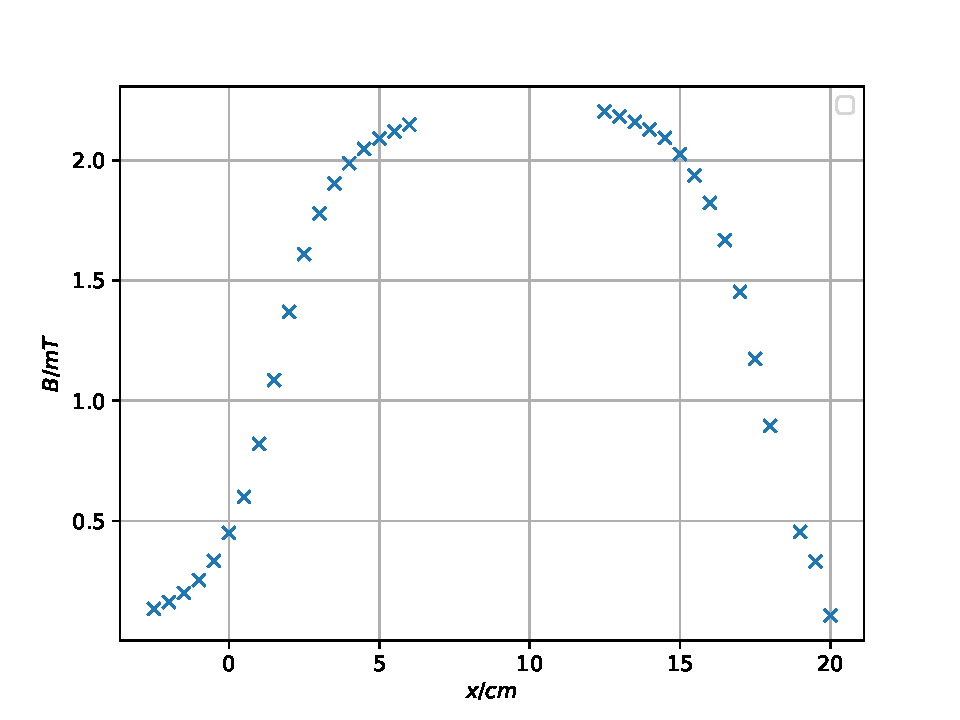
\includegraphics[width=\textwidth]{content/data/plot_long.pdf}
  \label{fig:long}
\end{figure}

\FloatBarrier
In der Tabelle \ref{tab:long} sind die gemessen Werte aufgefasst.
Dabei steht $x=0$ für den Anfang der Spule.
In der Abbildung \ref{fig:long} sind die Werte graphisch dargestellt.
Da aus technischen Gründen das Magnetfeld in der Mitte der Spule nicht gemessen werden konnte, wird näherungsweise der Messerte bei $\SI{6}{\centi\meter}$ genommen.
\begin{equation*}
  B(\SI{6}{\centi\meter}) = \SI{2.148}{\milli\tesla} 
\end{equation*}

Der nach \eqref{eqn:spule} berechnete Werte liegt bei:
\begin{equation*}
  B = \SI{1.9936}{\milli\tesla} 
\end{equation*}
Dabei ist $n=300$, die Stromstärke $I=\SI{1}{\ampere}$ und die Länge $l=\SI{18.9}{\centi\meter}$.

\FloatBarrier
\subsection{Kurze Spule}

\begin{table}
\centering
\caption{Messwerte der kurzen Spule.}
\begin{tabular}{cc|cc}
\toprule
$x \:/\: \si{\centi\meter}$ & $B \:/\: \si{\milli\tesla}$ &$x \:/\: \si{\centi\meter}$ & $B \:/\: \si{\milli\tesla}$ \\
\midrule
-2.5 & 0.079 & 4.5 & 1.817  \\
-2.0 & 0.104 & 5.0 & 1.751  \\
-1.5 & 0.177 & 5.5 & 1.634  \\
-1.0 & 0.239 & 6.0 & 1.451  \\
-0.5 & 0.326 & 6.5 & 1.196  \\
0.0 & 0.465  & 7.0 & 0.937  \\
0.5 & 0.650  & 7.5 & 0.678  \\
1.0 & 0.905  & 8.0 & 0.488  \\
1.5 & 1.194  &  8.5 & 0.343  \\
2.0 & 1.430  & 9.0 & 0.237  \\
2.5 & 1.618  & 9.5 & 0.181  \\
3.0 & 1.750  & 10.0 & 0.137 \\
3.5 & 1.818  & 10.5 & 0.110 \\
4.0 & 1.837  & 11.0 & 0.087 \\
\bottomrule
\label{tab:short}
\end{tabular}
\end{table}

\begin{figure}
  \centering
  \caption{Die Messwerte aus der Tabelle \ref{tab:short} grafisch aufgefasst.}
  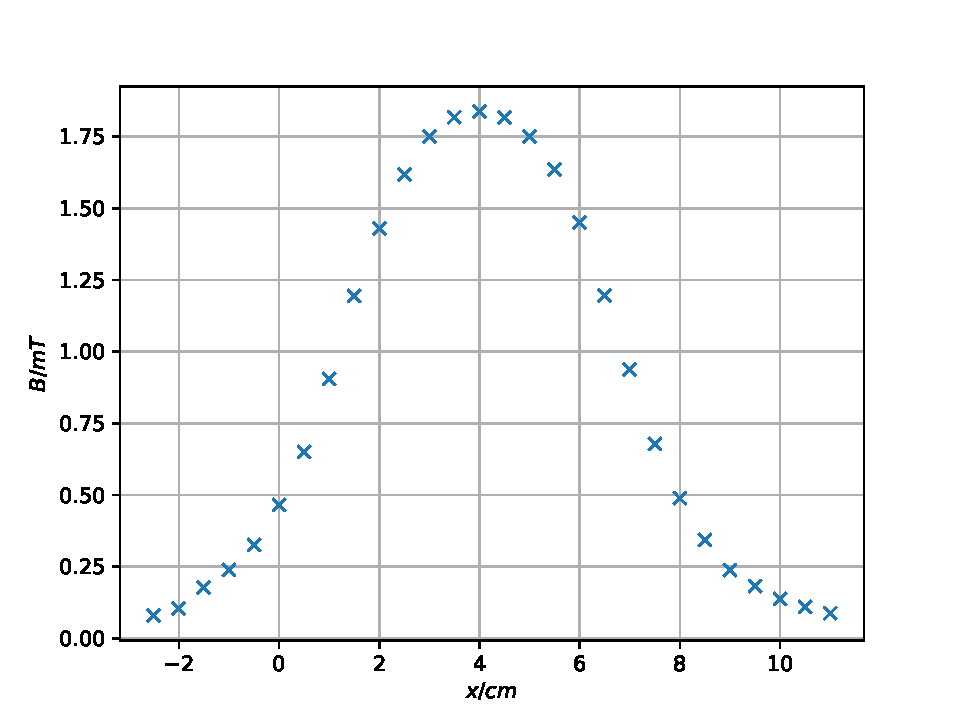
\includegraphics[width=\textwidth]{content/data/plot_short.pdf}
  \label{fig:short}
\end{figure}

Die Messwerte des Magnetfeldes der kurzen Spule sind in der Tabelle \ref{tab:short} zu sehen.
Die Werte sind anschließend in der Grafik \ref{fig:short} aufgetragen worden.
Das Magnetfeld in der Mitte der Spule hat nach Messung folgenden Wert
\begin{equation*}
  B(\SI{4}{\centi\meter})=\SI{1.837}{\milli\tesla} .
\end{equation*}
Der theoretisch berechnete Werte liegt wiederum bei
\begin{equation*}
  B = \SI{1.477}{\milli\tesla}
\end{equation*}
mit $I=\SI{1}{\ampere}$, $n=100$ und $l=\SI{8.5}{\centi\meter}$.
\FloatBarrier

\subsection{Helmholtzspulen}

Das Magnetfeld der Helmholtzspulen wurde für drei verschiedene Abstände gemessen.
Es wurden die Abstände $d_1=\SI{11}{\centi\metre}, d_2=\SI{7}{\centi\metre}$ und $d_3=\SI{15}{\centi\metre}$ gewählt.
Dabei ergab die Messung für den Abstand $d_1$, die Werte in Tabelle \ref{tab:helm1}.
Die Werte in Tabelle \ref{tab:helm2} sind bei der Messung für Abstand $d_2=\SI{7}{\centi\metre}$ aufgenommen worden.
Die Messung bei Abstand $d_3=\SI{15}{\centi\metre}$ ergaben die Werte in Tabelle \ref{tab:helm3}.
Die Werte in den Tabellen wurden in den Graphiken \ref{fig:helm1} für $d_1$, \ref{fig:helm2} für $d_2$ und \ref{fig:helm3} für $d_3$ dargstellt.

Alle Theoriewerte wurden mit einer Stromstärke von $I=\SI{2.5}{\ampere}$, einer Windungszahl von $n=100$ und einem Spulendurchmesser von $d=\SI{0.125}{\meter}$ berechnet.
Bei dem Spulenpaar mit Abstand $d_1$ wurde in der Mitte der beiden Spulen eine Feldstärke von 
\begin{equation*}
  B(\SI{5.5}{\centi\meter}) =\SI{2.755}{\milli\tesla}
\end{equation*}
gemessen.
Der nach Gleichung \eqref{eqn:helm} berechnete Theoriewert beträgt dabei
\begin{equation*}
  B_1=\SI{2.241}{\milli\tesla} .
\end{equation*}
Beim Abstand $d_2$ konnte das Magnetfeld nicht in der Mitte der Spulen gemessen werden.
Deswegen wird der Wert für $x=\SI{2}{\centi\meter}$
\begin{equation*}
  B(\SI{2}{\centi\meter})=\SI{3.841}{\milli\tesla}
\end{equation*}
mit dem Theoriewert verglichen, welcher mit der Formel \eqref{eqn:helm} berechnet wurde und 
\begin{equation*}
  B_2 =\SI{3.255}{\milli\tesla}
\end{equation*}
beträgt.
Für den Abstand $d_3$ hat das Magnetfeld in der Mitte der Spulen eine Stärke von 
\begin{equation*}
  B(\SI{8}{\centi\meter})=\SI{1.919}{\milli\tesla} .
\end{equation*}
Der Theoriewert beträgt dabei 
\begin{equation*}
  B_3=\SI{2.656}{\milli\tesla}.
\end{equation*}

\FloatBarrier
\begin{table}
\centering
\caption{Messwerte der Helmholtzspulen mit Abstand $d_1=11\si{\centi\meter}$.}
\begin{tabular}{cc}
\toprule
$x \:/\: \si{\centi\meter}$ & $B \:/\: \si{\milli\tesla}$ \\
\midrule
1.0 & 2.847 \\
1.5& 2.767\\
2.0& 2.701\\
2.5& 2.646\\
3.0& 2.610\\
3.5& 2.594\\
4.0& 2.601\\
4.5& 2.638\\
5.0& 2.690\\
5.5& 2.755\\
6.0& 2.836\\
12.0& 2.356\\
13.0& 2.002\\
14.0& 1.640\\
15.0& 1.336\\
16.0& 1.077\\
\bottomrule
\label{tab:helm1}
\end{tabular}
\end{table}

\begin{table}
\centering
\caption{Messwerte der Helmholtzspulen mit Abstand $d_2=\SI{7}{\centi\metre}$.}
\begin{tabular}{cc}
\toprule
$x \:/\: \si{\centi\metre}$ & $B \:/\: \si{\milli\tesla}$ \\
\midrule
1.0& 3.836  \\
1.1& 3.838\\
1.2& 3.837\\
1.3& 3.838\\
1.4& 3.837\\
1.5& 3.838\\
1.6& 3.839\\
1.7& 3.839\\
1.8& 3.840\\
1.9& 3.839\\
2.0& 3.841\\
2.1& 3.841\\
2.2& 3.842\\
2.3& 3.846\\
8.0& 2.534\\
9.0& 2.194\\
10.0& 1.781\\
11.0& 1.463\\
12.0& 1.188\\
\bottomrule
\label{tab:helm2}
\end{tabular}
\end{table}

\begin{table}
\centering
\caption{Messwerte der Helmholtzspulen mit Abstand $d_3=\SI{15}{\centi\metre}$.}
\begin{tabular}{cc}
\toprule
$x \:/\: \si{\centi\metre}$ & $B \:/\: \si{\milli\tesla}$ \\
\midrule
1& 2.423  \\
2& 2.155\\
3& 1.927\\
4& 1.753\\
5& 1.668\\
6& 1.665\\
7& 1.753\\
8& 1.919\\
9& 2.149\\
10& 2.418\\
16& 2.229\\
17& 1.899\\
18& 1.561\\
19& 1.262\\
20& 1.015\\
\bottomrule
\label{tab:helm3}
\end{tabular}
\end{table}

\begin{figure}
\centering
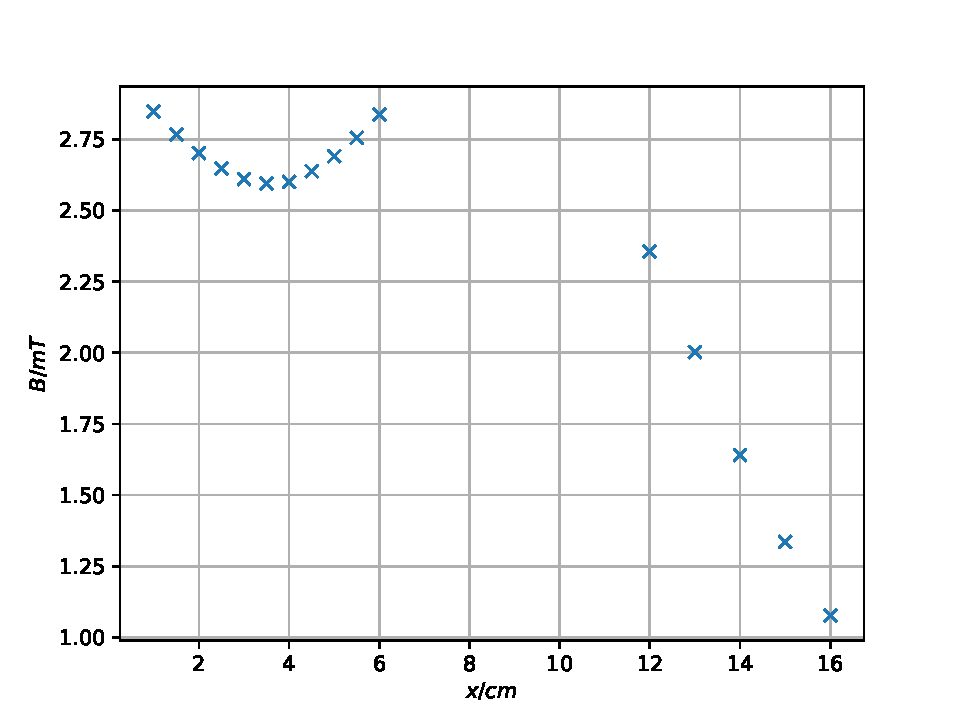
\includegraphics{content/data/plot_helmholtz1.pdf}
\caption{B-Feld in Abhängigkeit vom Ort $x$ mit dem Spulenabstand $d_1=\SI{11}{\centi\metre}$. }
\label{fig:helm1}
\end{figure}

\begin{figure}
\centering
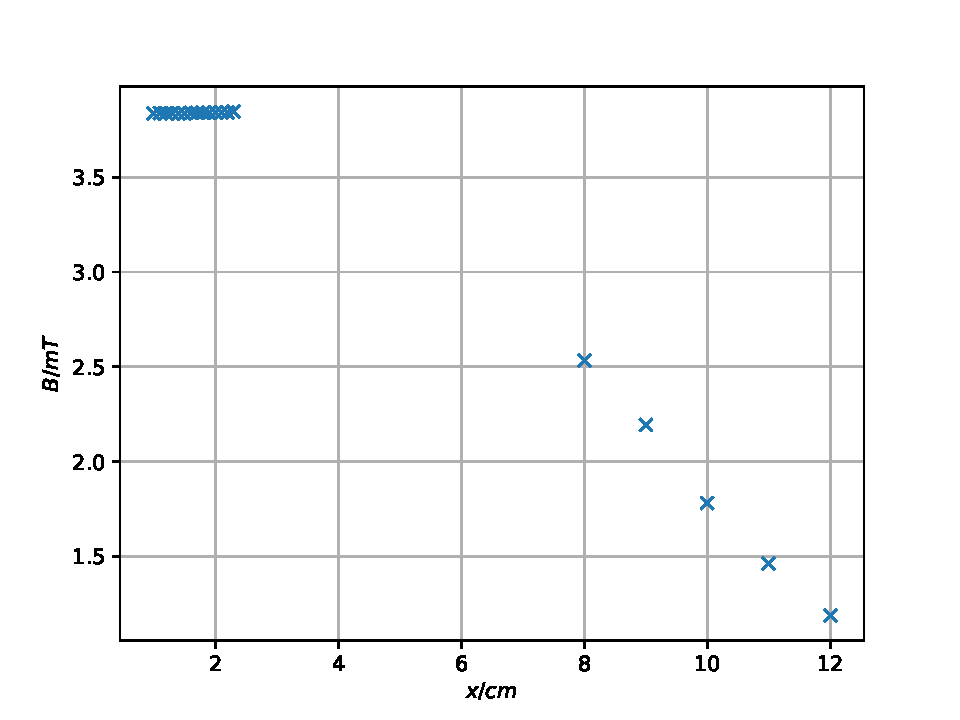
\includegraphics{content/data/plot_helmholtz2.pdf}
\caption{B-Feld in Abhängigkeit vom Ort $x$ mit dem Spulenabstand $d_2=\SI{7}{\centi\metre}$.}
\label{fig:helm2}
\end{figure}

\begin{figure}
\centering
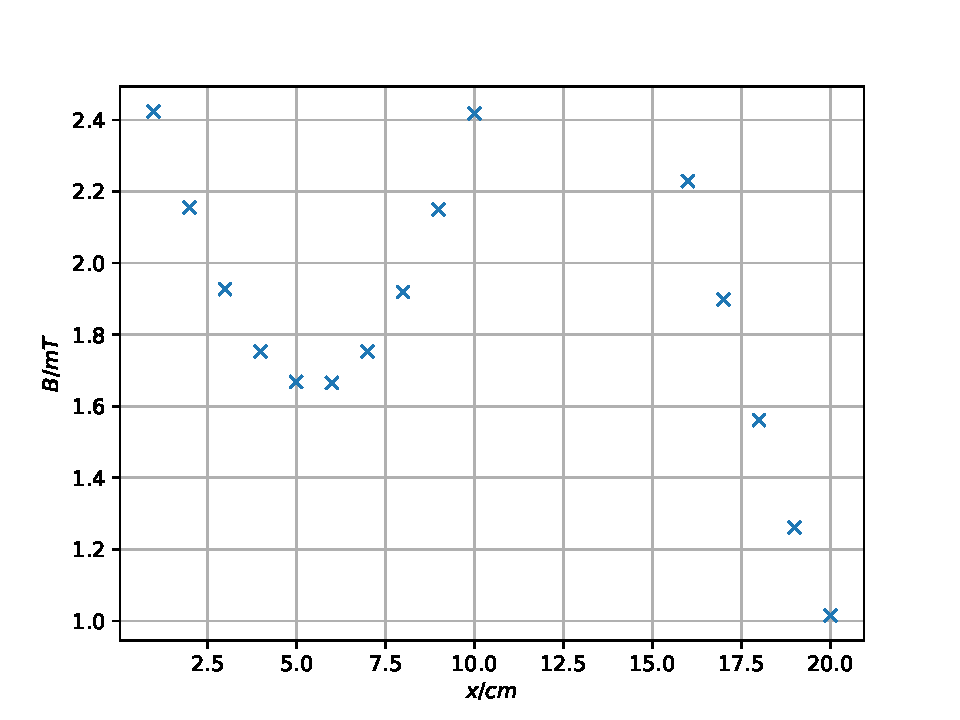
\includegraphics{content/data/plot_helmholtz3.pdf}
\caption{B-Feld in Abhängigkeit vom Ort $x$ mit dem Spulenabstand $d_3=\SI{15}{\centi\metre}$.}
\label{fig:helm3}
\end{figure}

\FloatBarrier
\subsection{Hysteresekurve}

\begin{table}
\centering
\caption{Messwerte der Ringspule mit Eisenkern.}
\begin{tabular}[t]{cc}
\toprule
$I \:/\: \si{\ampere}$ & $B \:/\: \si{\milli\tesla}$ \\
\midrule
0& 0\\
1& 162  \\
2& 341\\
3& 443\\
4& 512\\
5& 563\\
6& 605\\
7& 642\\
8& 674\\
9& 705\\
10& 730\\
9& 710\\
8& 692\\
7& 670\\
6& 645\\
5& 614\\
4& 577\\
3& 528\\
2& 462\\
1& 335\\
0& 129\\
-1& -073\\
-2& -258\\
-3& -390\\
-4& -483\\
-5& -549\\
-6& -598\\
-7& -639\\
-8& -672\\
-9& -703\\
-10& -730\\
\bottomrule
\end{tabular}
\begin{tabular}[t]{cc}
\toprule
$I \:/\: \si{\ampere}$ & $B \:/\: \si{\milli\tesla}$ \\
\midrule
-9& -712\\
-8& -693\\
-7& -672\\
-6& -646\\
-5& -616\\
-4& -580\\
-3& -533\\
-2& -468\\
-1& -335\\
0& -126\\
1& 70\\
2& 251\\
3& 389\\
4& 481\\
5& 545\\
6& 593\\
7& 633\\
8& 667\\
9& 697\\
10& 723\\
\bottomrule
\end{tabular}
\label{tab:ring}
\end{table}

\begin{figure}
\centering
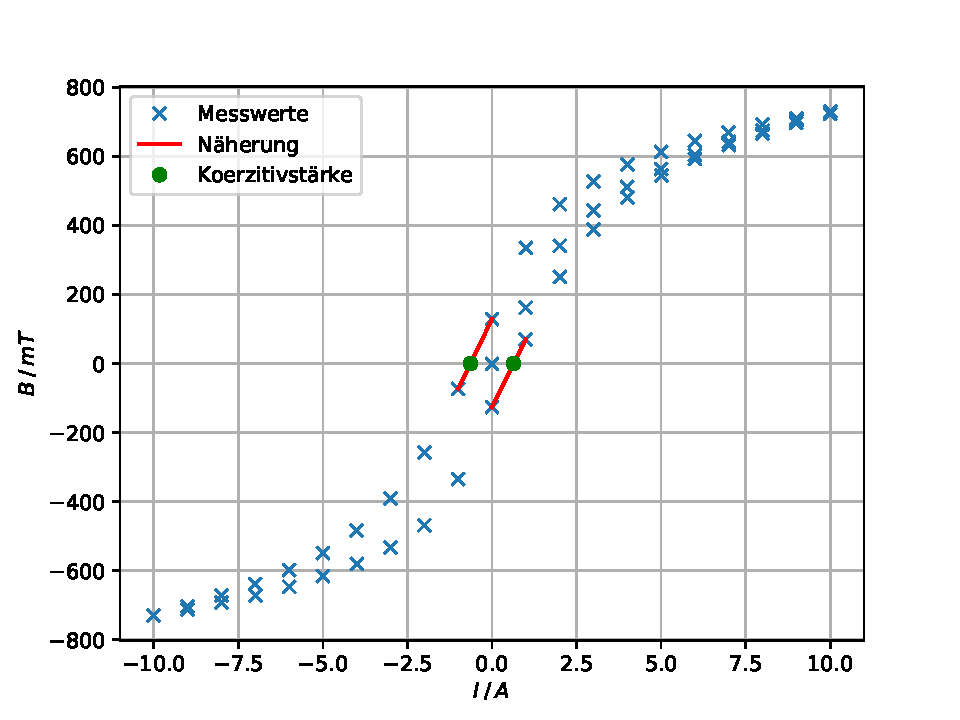
\includegraphics[width=\textwidth]{content/data/plot_ring.pdf}
\caption{Die Hysteresekurve.}
\label{fig:ring}
\end{figure}

In der Tabelle \ref{tab:ring} sind die Messwerte aufgetragen die beim messen des Magnetfeldes der Ringspule aufgenommen wurden.
Daraufhin wurde eine Hysteresekurve mit den Werten erstellt die in Abbildung \ref{fig:ring} zu sehen ist.
Zu erkennen ist dabei, dass die Remanenz $B_\text{r}$ bei 
\begin{equation*}
  B_\text{r} =\SI{129}{\milli\tesla}
\end{equation*}
liegt.
In der Graphik \ref{fig:ring} ist außerdem die Koerzitivfeldstärke $H_\text{c}$ aufgetragen.
Diese liegt bei einem Wert von
\begin{equation*}
  H_\text{c} =\SI{0.638}{\ampere}.
\end{equation*}
